\subsection{Protecting the blocks}
\label{sect:repudiation}
The blocks have to be cryptographically protected and validated.
Tampering with the contents of blocks should be detectable and useless.
In part this is already done by using the hashes as pointers in subsequent blocks.
If a block in a chain is changed, then the subsequent hash pointers will become invalid~\cite{VanderLubbe-crypto}.
The chain becomes detached.

A second issue is that peers should not be able to deny conducting a transaction.
This will prevent a peer to be able to deny his freeriding if this is transcibed in his chain.
Both peers sign the block using their private keys to acknowledge that the transaction has happened.
This signature is added to the block.

In a transaction between peer A and peer B, the whole block is not signed by every peer.
Peer A can only make valid claims about, and have authority, over the interaction between peers
and his own total up and download amounts.
So A does not need to sign the data containing the previous hash and the total up and down of the other peer B.
These amounts can be verified using the chain of peer B.
The parts of what is signed by peer A and what is signed by B can be seen in Figure \ref{fig:signatures}.
\begin{figure}
	\centerline{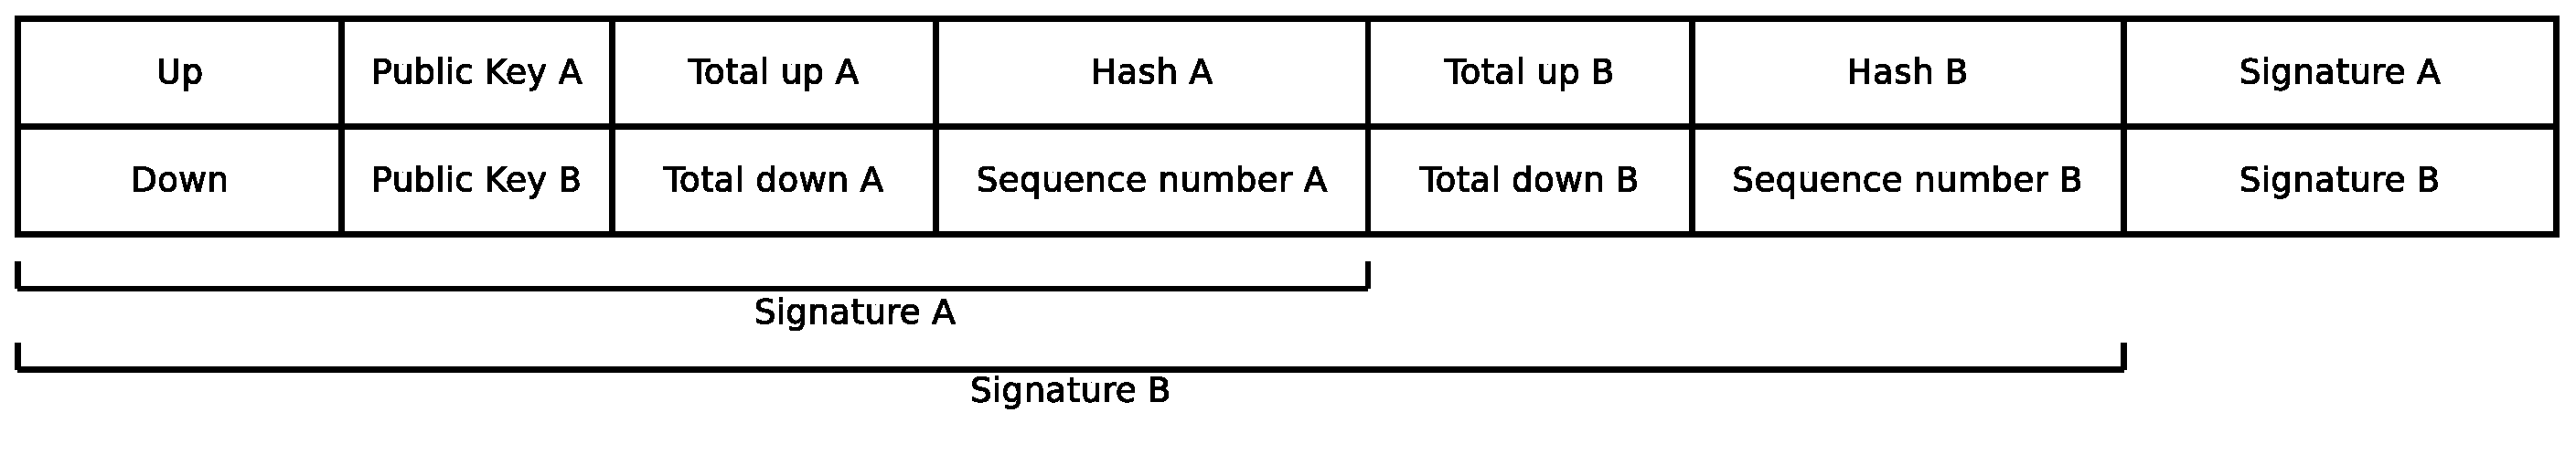
\includegraphics[scale=0.3]{design/figs/signatures.eps}}
	\caption{Fields protected by each of the two signatures.}
	\label{fig:signatures}
\end{figure}

Digital signatures have the property to be non-repudiable of origin~\cite{VanderLubbe-crypto}.
After signing a block the signer cannot later deny providing his signature.
Only with the possesion of a secret key,
a signature can be made;
so only the signer could have made the signature.
This is assuming the secret key was not comprimised.
The blocks become durable records and are irrevokable and irrefutable.
Because peers cannot repudiate their own signature.

